Archie utilizes information retrieval and machine learning techniques to automatically detect architectural decisions from source code. The detection engine implements a set of classification techniques and each classifier is trained using code snippets representing different architectural tactics collected from hundreds of high-performance, open-source projects~\cite{FSE2012,ICSE2012,Dissertation}. In the training phase the classifiers learn the terms, method and variable names, and development APIs that developers typically use to implement each tactic. These terms are used during the classification phase to calculate the likelihood that any given source file implements a tactic. The accuracy of the tactical spike detection technique is evaluated through several experiments which indicate our technique is capable of returning reliable results. The details of our detection engine, the classification formula and accuracy metrics are described in several previous works~\cite{Dissertation,ICSE2012}. 

\begin{figure}[tbph]
\centering
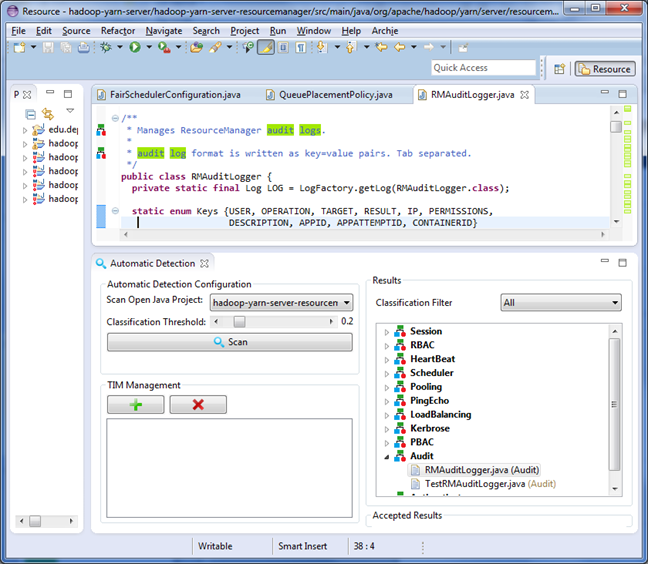
\includegraphics[width=0.9\linewidth]{./Detect}
\caption{Detected Tactical Spikes in Apache Hadoop Yarn Project}
\label{fig:Detect}
\end{figure}

Figure~\ref{fig:Detect} shows a screenshot of Archie where the classifiers are launched against the code in an Eclipse project. Several different architectural tactics are discovered in the source code of the Apache Hadoop Yarn project and categorized based on tactic type. Each category includes all the source files contributing to the implementation of each tactic. Furthermore, Archie highlights the method names, APIs and comments related to the tactic. For example, in Figure~\ref{fig:Detect} comments about audit trails are highlighted which helps developers understand why this file is considered tactical.

This feature will help developers to better understand the current state of implemented tactical spikes. This is especially useful when a new developer joins the team and they need to quickly comprehend the architectural choices behind the source code or when developers alter a new module of software which they have not worked on previously. Furthermore, this auto-detection engine can assist developers in more easily documenting their previous tactical spikes. Initially they can detect and recover architectural tactics in the source code, and then use the previously described feature of TTPs and connect these source files into a visual and informative representation of tactics. The visualization and documentation of tactical spikes as TTPs increases program comprehension and design communication which significantly reduces the effort to maintain such models compared to traditional approaches.